% ============================================================
%  CATÉTERES VENOSOS CENTRALES
%  Licenciatura en Imagenología --- UdelaR
%  Imagenología Especializada I
%  Lic. Germán Boz --- 2025
% ============================================================

\chapter{Catéteres venosos centrales}

	

% ============================================================
%  PUNTOS CLAVE PARA EL EXAMEN ORAL
% ============================================================
\begin{cajakeypoints}
	\textbf{\color{azulprincipal} Puntos clave para el examen oral}
	\begin{itemize}[noitemsep, topsep=2pt]
		\item Los CVC son accesos venosos para tratamientos terapéuticos, medicamentos y hemodiálisis.
		\item Clasificación principal: VVC, catéter doble luz, catéter tunelizado (Hickman), catéter gemelar, Port-a-Cath y FAV.
		\item La punta del catéter debe quedar a nivel de la carina (unión VCS--aurícula derecha).
		\item Posición demasiado proximal (1/3 superior VCS / tronco braquiocefálico) aumenta riesgo de trombosis; dentro de aurícula genera arritmia y riesgo de perforación.
		\item Distribución de sala: paciente en decúbito dorsal (Trendelenburg en CDL); arco en C ingresa contralateral al lado de punción; monitores a los pies.
		\item Protocolo básico (Seldinger): punción ecoguiada $\to$ guía $\to$ dilatador $\to$ catéter $\to$ control RX de punta.
		\item Complicaciones: kinking, catéter pellizcado, neumotórax, hemotórax.
		\item El filtro de VCI se coloca infrarenal, identificando las venas renales con medio de contraste antes de liberar el dispositivo.
	\end{itemize}
\end{cajakeypoints}

\vspace{1em}

% ============================================================
%  SECCIÓN 1 --- DEFINICIÓN
% ============================================================
\section*{Definición}

\begin{cajadefinicion}
	Los \textbf{catéteres venosos centrales (CVC)} son accesos venosos de largo recorrido que se insertan en venas de grueso calibre y cuya punta queda alojada en la vena cava superior o en la aurícula derecha, permitiendo la administración de tratamientos terapéuticos, medicamentos, quimioterapia y la realización de hemodiálisis.
\end{cajadefinicion}

Se indican cuando el paciente tiene venas frágiles o de difícil acceso, cuando el tratamiento se prevé de varios días a meses, cuando las venas han sido dañadas por tratamientos previos, cuando se requieren fármacos vesicantes (como citostáticos) o cuando se necesitan múltiples infusiones simultáneas.

\clearpage
% ============================================================
%  SECCIÓN 2 --- CLASIFICACIÓN
% ============================================================
\section*{Clasificación}

\subsection*{Tipos de catéteres venosos centrales}

{\renewcommand{\arraystretch}{1.3}
	\begin{center}
		\begin{tabular}{|>{\bfseries}p{3.2cm}|p{5cm}|p{5.5cm}|}
			\hline
			\textbf{Tipo} & \textbf{Características} & \textbf{Uso principal} \\
			\hline
			Vía Venosa Central (VVC) & Sonda flexible; yugular ext./int. o subclavia; termina en VCS. Puede ser radiopaca o radiolúcida. & Emergencia / CTI. Control con RX portátil o arco en C. \\
			\hline
			Catéter Doble Luz (CDL) & Transitorio, corta duración. Radiopaco. Extremo distal a nivel de aurícula derecha (carina). & Hemodiálisis de corto plazo. Mayor riesgo de infección. \\
			\hline
			Catéter Tunelizado (Hickman) & Silicona, subcutáneo, radiopaco. Túnel entre entrada venosa y salida cutánea. & Hemodiálisis de largo plazo. Menor riesgo de infección. \\
			\hline
			Catéter Gemelar & Dos catéteres independientes; dos sitios de punción; puntas a diferente altura. & Hemodiálisis cuando no es posible CDL único. \\
			\hline
			Port-a-Cath & Implantable con reservorio de silicona en bolsillo pre-pectoral. Radiopaco. & Terapias intermitentes prolongadas (quimioterapia). \\
			\hline
			FAV Nativa & Anastomosis quirúrgica arteria--vena con vena propia del paciente. & Hemodiálisis. Opción ideal. \\
			\hline
			FAV Protésica & Anastomosis con injerto vascular sintético. & Hemodiálisis cuando no es viable FAV nativa. Mayor riesgo infeccioso. \\
			\hline
		\end{tabular}
	\end{center}
}

% ============================================================
%  SECCIÓN 3 --- DISTRIBUCIÓN DE LA SALA Y POSICIONAMIENTO
% ============================================================
\section*{Distribución de la Sala y Posicionamiento}

El procedimiento puede realizarse tanto en block quirúrgico como en sala de hemodinámica. La mesa debe ser \textbf{radiolúcida en la región del tórax}.

\subsection*{Posición del paciente}

El paciente se coloca en \textbf{decúbito dorsal}. Para la colocación del catéter doble luz se utiliza habitualmente la posición de \textbf{Trendelenburg}, que facilita la punción y reduce el riesgo de embolia aérea.

\subsection*{Posición del equipo médico y del arco en C}

{\renewcommand{\arraystretch}{1.3}
	\begin{center}
		\begin{tabular}{|>{\bfseries}p{4cm}|p{9.5cm}|}
			\hline
			\textbf{Integrante / Equipo} & \textbf{Ubicación} \\
			\hline
			Cirujano y ayudante & A la cabecera del paciente, del lado derecho o izquierdo según el sector a puncionar. Excepción: catéter femoral (se ubican a nivel inguinal). \\
			\hline
			Instrumentista & Del mismo lado que el cirujano. \\
			\hline
			Arco en C & Ingresa \textbf{perpendicular} al paciente por el lado \textbf{contralateral} al sector a puncionar. \\
			\hline
			Monitores & A los pies del paciente. \\
			\hline
		\end{tabular}
	\end{center}
}

% ============================================================
%  SECCIÓN 4 --- PROCEDIMIENTO POR TIPO DE CATÉTER
% ============================================================
\section*{Procedimiento}

\subsection*{Catéter Doble Luz (CDL)}

La técnica sigue la \textbf{secuencia de Seldinger}:

\begin{enumerate}[noitemsep]
	\item Punción del vaso (yugular interna/externa, subclavia o femoral) bajo \textbf{guía ecográfica}.
	
	\begin{figure}[h]
		\centering
		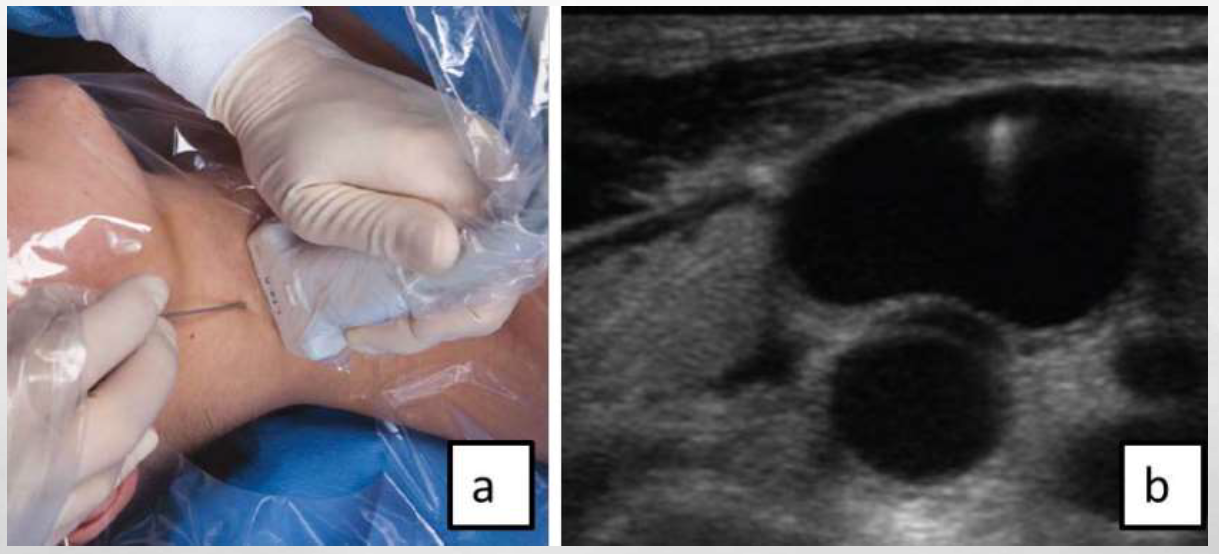
\includegraphics[width=0.7\linewidth]{imagenes/puncion_ecoguiada}
		\caption[Puncion Guiada]{}
		\label{fig:puncionecoguiada}
	\end{figure}
		
	\item Pasaje de \textbf{guía metálica} a través de la aguja; control con RX en región mediastinal.
	
	\begin{figure}[h]
		\centering
		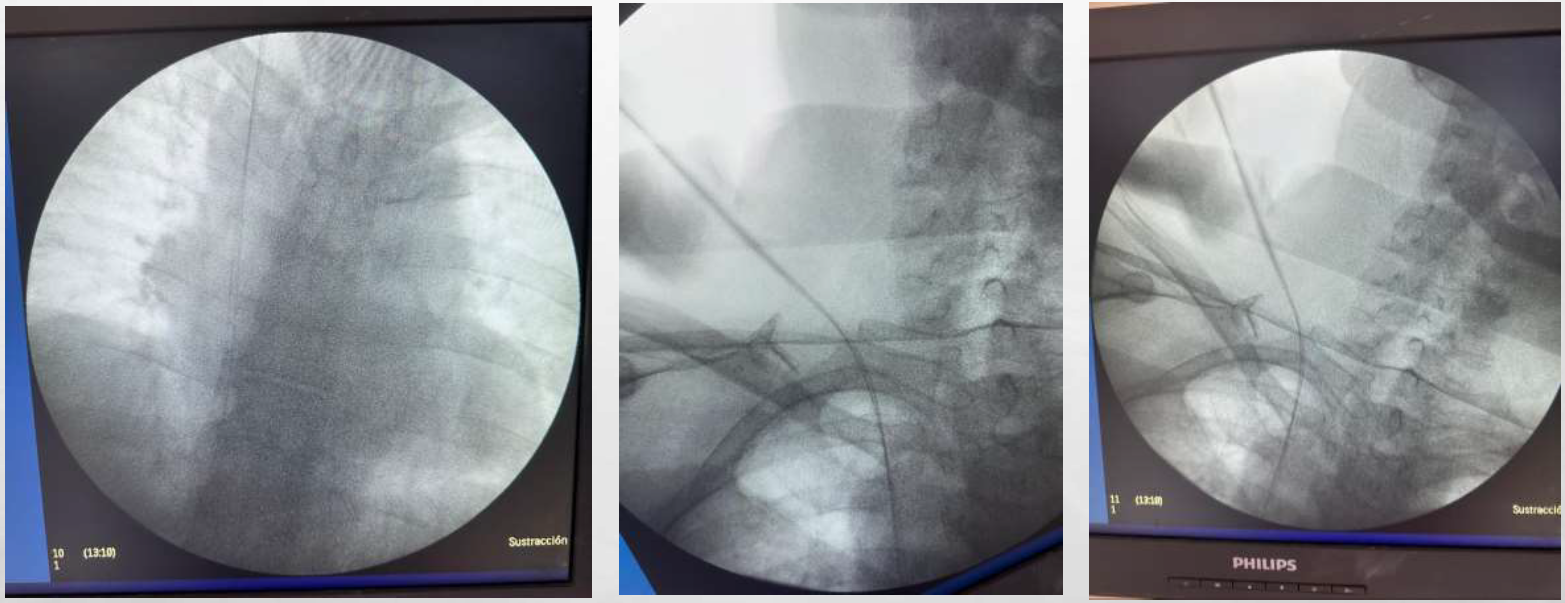
\includegraphics[width=0.7\linewidth]{imagenes/guias_dilatador}
		\caption[Guías y dilatadores]{}
		\label{fig:guiasdilatador}
	\end{figure}
		
	\item Dilatación del acceso venoso con control RX en zona de punción.
	\item Colocación del CDL sobre la guía hasta posición correcta; retirada de la guía con control RX.

	\begin{figure}[h]
		\centering
		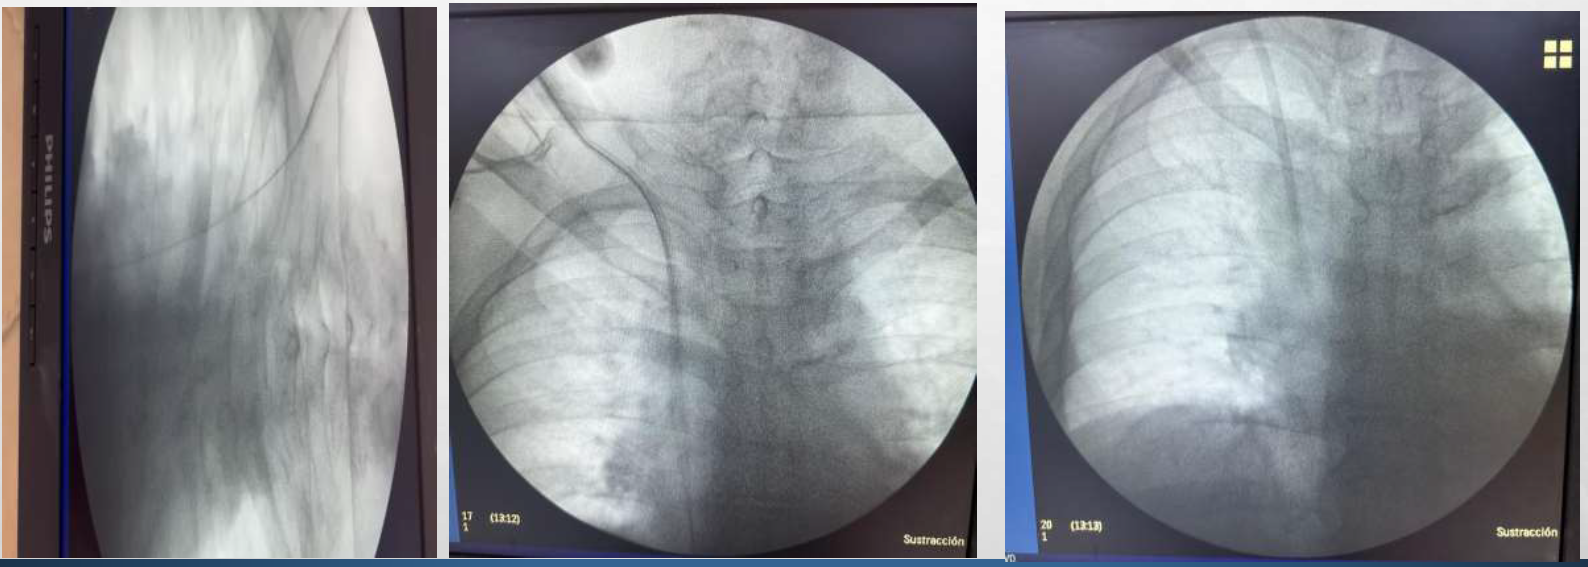
\includegraphics[width=0.7\linewidth]{imagenes/retiro _guia}
		\caption[Retiro de guía]{}
		\label{fig:retiro-guia}
	\end{figure}
	
	
	\item Control final de la \textbf{punta del catéter} en mediastino (nivel de carina / unión VCS--AD).
	\item Prueba de funcionamiento de ambas ramas del catéter.
\end{enumerate}

\subsection*{Catéter Tunelizado (Hickman)}

La fase inicial es idéntica al CDL. Una vez confirmada la posición de la guía, el cirujano realiza adicionalmente:

\begin{enumerate}[noitemsep]
	\item Creación del \textbf{túnel subcutáneo} desde el sitio de punción venosa hasta la salida cutánea planificada.
	\item Pasaje del catéter de silicona por el túnel.
	\item Control radiológico secuencial: guía $\to$ curva $\to$ punta (a nivel de VCS / unión AD).
	
	
	\begin{figure}[h]
		\centering
		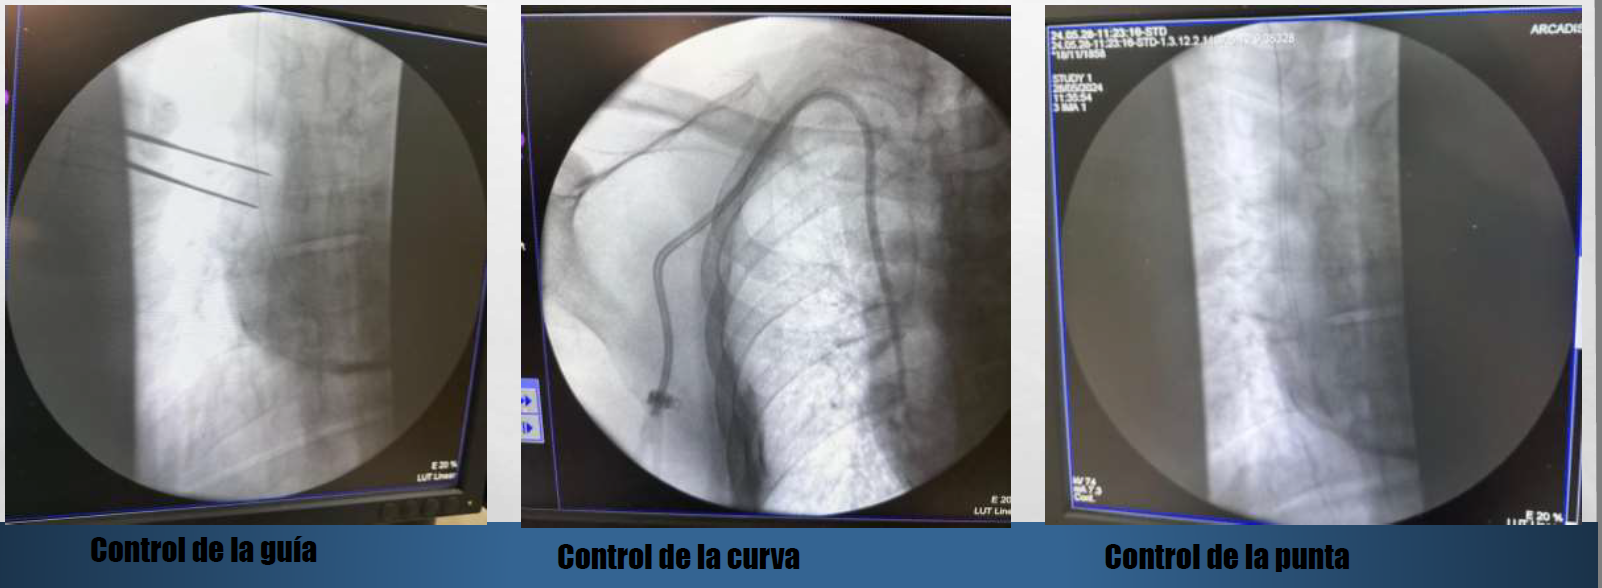
\includegraphics[width=0.7\linewidth]{imagenes/tunelizado_hickman}
		\caption[Controles]{}
		\label{fig:tunelizadohickman}
	\end{figure}
	
	\begin{figure}[h]
		\centering
		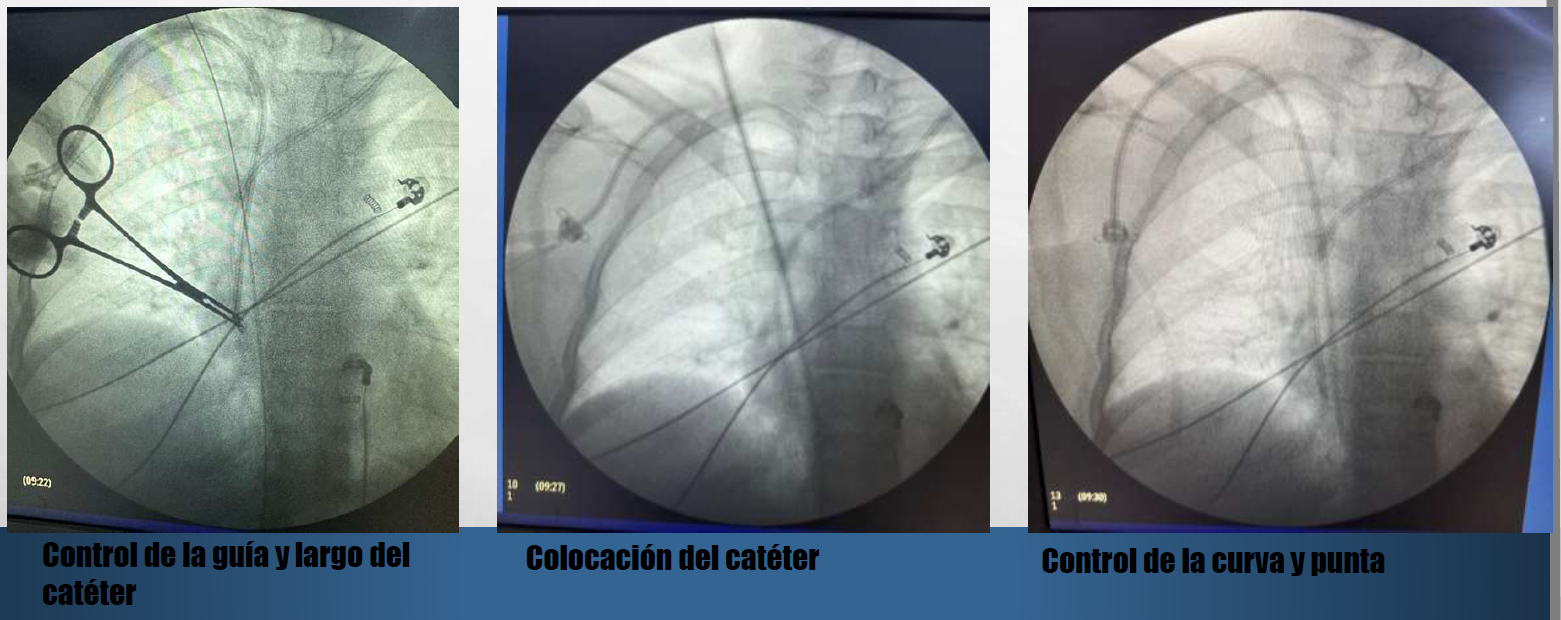
\includegraphics[width=0.7\linewidth]{imagenes/tunelizado_hickman2}
		\caption{}
		\label{fig:tunelizadohickman2}
	\end{figure}
	
\end{enumerate}

\subsubsection{Ubicación de la punta del catéter:}

\begin{itemize}
	\item Se controla por Rx en la vena Cava superior a nivel de la Carina o de unión entre la vena Cava superior y Aurícula derecha.
	
	\item La localización 1/3 superior de vena Cava superior y tronco Braquiocefálico, se asocia a riesgos de trombosis.
	
	\item Dentro de la aurícula puede ocasionar arritmia, trombosis o perforación cardíaca si esta por tiempo prolongado
\end{itemize}

\subsection*{Catéter Gemelar}

Se realizan \textbf{dos punciones independientes} en el mismo vaso. Se colocan dos guías simultáneamente, se controla la posición de ambas, se dilatan los accesos y se insertan los catéteres con las \textbf{puntas a diferente altura} para evitar recirculación.

\begin{figure}[h]
	\centering
	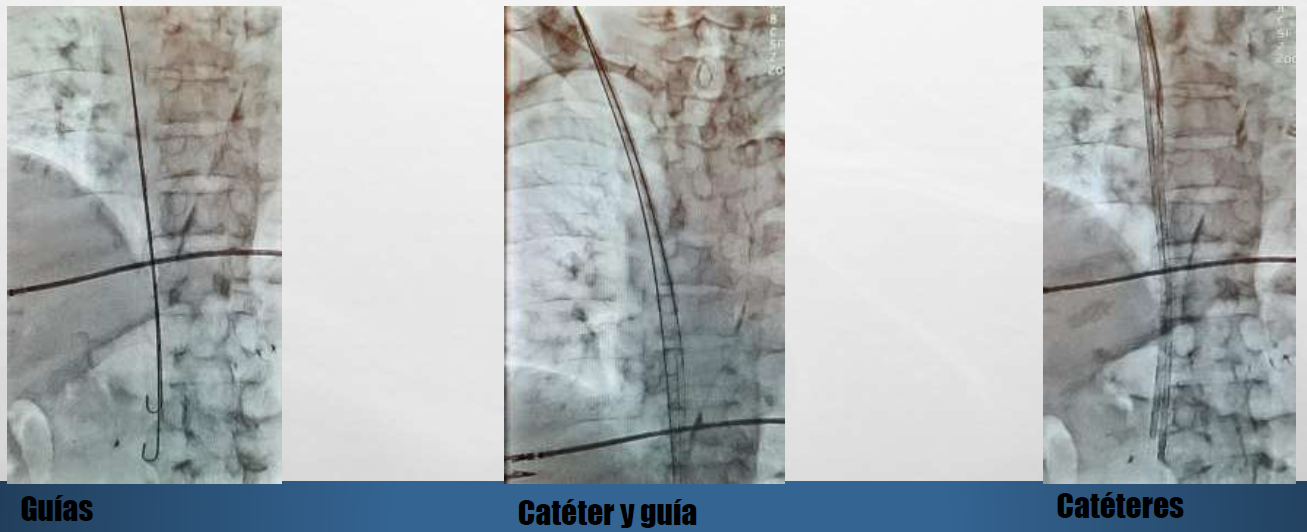
\includegraphics[width=1\linewidth]{imagenes/gemelar1}
	\caption{}
	\label{fig:gemelar1}
\end{figure}

\begin{figure}[h]
	\centering
	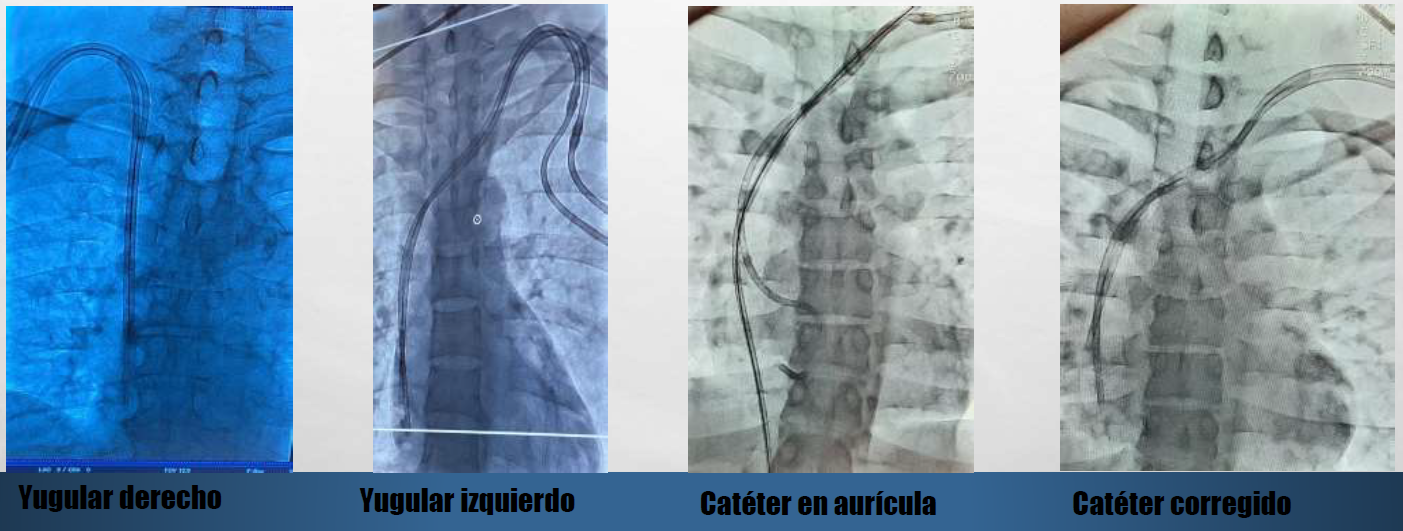
\includegraphics[width=1\linewidth]{imagenes/gemelar2}
	\caption{}
	\label{fig:gemelar2}
\end{figure}



\subsection*{Port-a-Cath}

\begin{enumerate}[noitemsep]
	\item Fase inicial idéntica al CDL (punción, guía, dilatación).
	\item El cirujano realiza un \textbf{bolsillo subcutáneo} en la región del pectoral mayor para alojar el reservorio.
	\item El catéter se tuneliza por vía subcutánea desde el bolsillo hasta el sitio de punción venosa y se conecta al reservorio.
	\item Control radiológico de punta y curvatura para confirmar que el catéter \textbf{no colapse}.
\end{enumerate}


\begin{figure}[h]
	\centering
	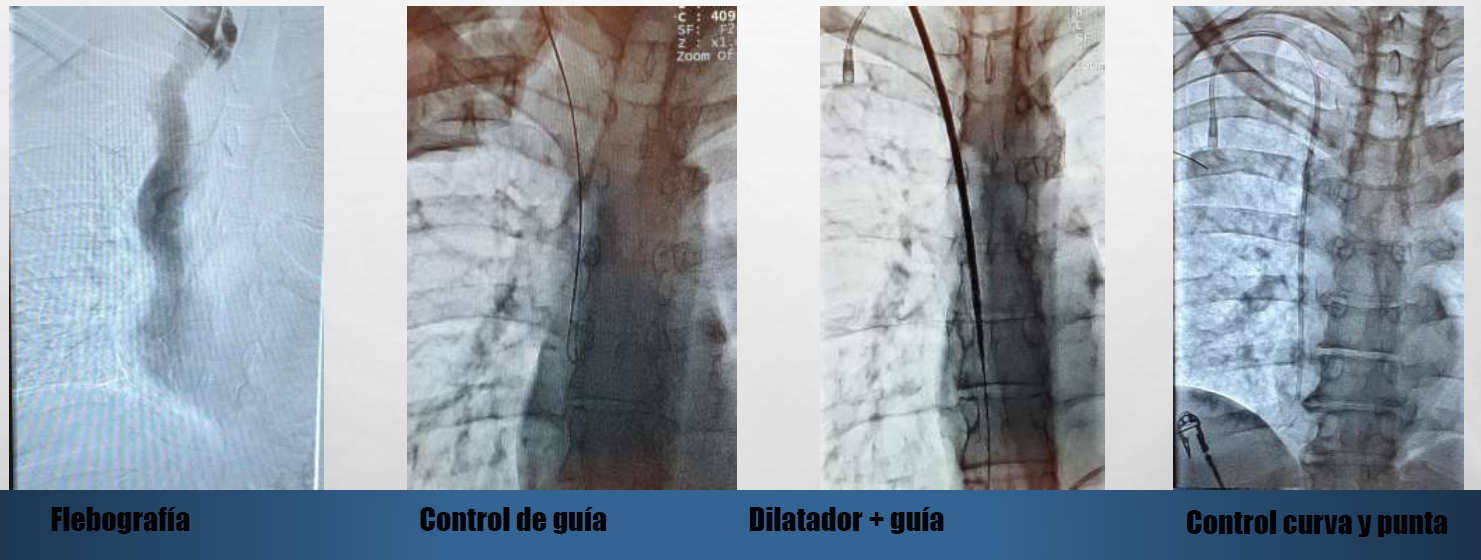
\includegraphics[width=1\linewidth]{imagenes/portacath}
	\caption{}
	\label{fig:portacath}
\end{figure}


\subsubsection{Complicaciones:}
\begin{itemize}
	\item kinking (angulo cerrado de la curva).
	\item Catéter pellizcado.
	\item Neumotorax.
	\item Hemotorax.
\end{itemize}

\clearpage


% ============================================================
%  SECCIÓN 6 --- FISTULOGRAFÍA
% ============================================================
\section*{Fistulografía (FAV)}

Cuando una FAV deja de funcionar (obstrucción), el licenciado en imagenología interviene realizando una \textbf{fistulografía diagnóstica}:

\begin{itemize}[noitemsep]
	\item Adquisición en \textbf{DSA} a 3--6 imágenes/segundo; se aumenta la cadencia para evaluar la dinámica de flujo.
	\item La mayoría de las FAV son \textbf{humerocefálicas o humerobasílicas}; se realizan \textbf{dos enfoques de frente}:
	\begin{enumerate}[noitemsep]
		\item Desde el \textbf{pliegue del codo} (mostrando la aguja de punción) hasta la \textbf{axila inclusive}.
		\item Desde la \textbf{axila} hasta la desembocadura de la VCS en la aurícula derecha.
	\end{enumerate}
	\item Realizado el diagnóstico, el \textbf{cirujano vascular} evaluará el tratamiento (angioplastia, revisión quirúrgica, etc.).
\end{itemize}


\begin{figure}[h]
	\centering
	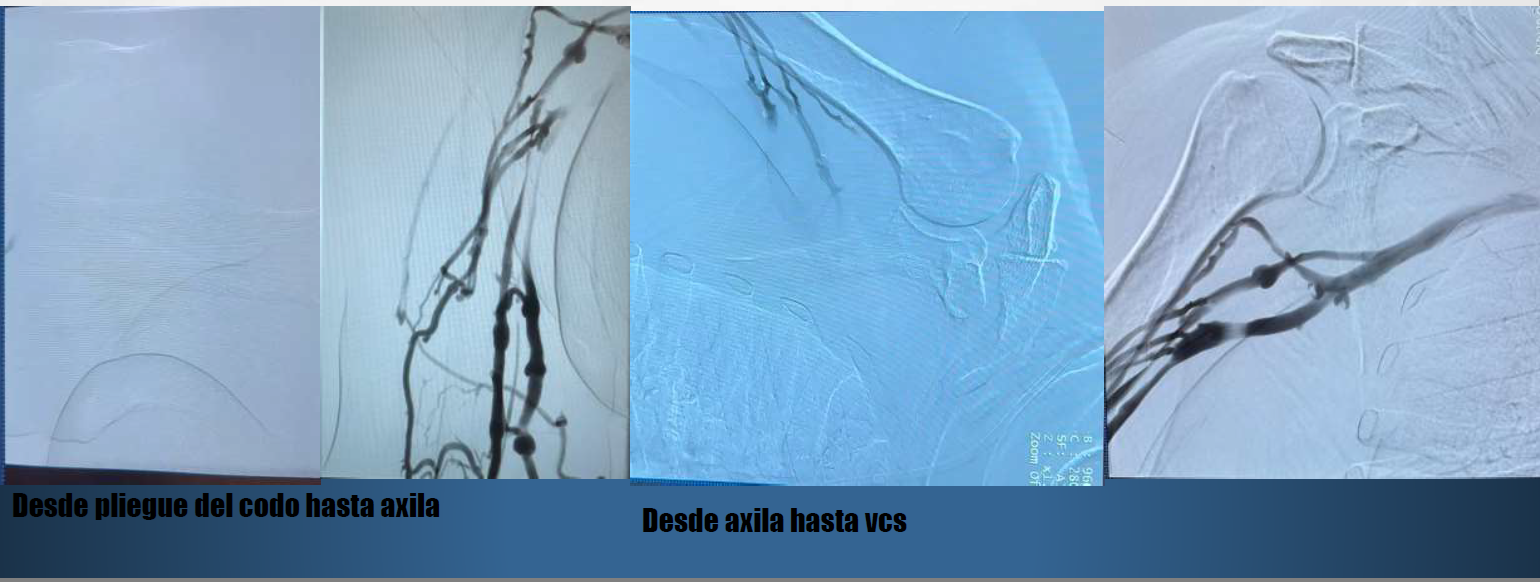
\includegraphics[width=1\linewidth]{imagenes/fistulo}
	\caption{}
	\label{fig:fistulo}
\end{figure}



\subsection*{Filtro de Vena Cava Inferior (FVCI)}

Dispositivo mecánico implantado para \textbf{prevenir embolismos pulmonares} cuando no es posible una anticoagulación adecuada. Los trombos, generados en venas de MMSS o MMII, pueden migrar hacia los pulmones provocando disnea, dolor torácico o muerte.

\begin{enumerate}[noitemsep]
	\item Acceso por vía \textbf{yugular o femoral}; avance de guía hasta VCI abdominal.
	\item Inyección de \textbf{medio de contraste yodado} para identificar la altura de las \textbf{venas renales} (marca en sustracción DSA).
	\item Avance del sistema liberador hasta posición \textbf{infrarenal}.
	\item Liberación del filtro: se expande y ancla a la pared del vaso.
	\item Control final de ubicación con RX.
\end{enumerate}


\clearpage
% ============================================================
%  CIERRE --- ESQUEMA MENTAL FINAL
% ============================================================
\section*{Esquema Mental --- Repaso Final}

\begin{cajakeypoints}
	\begin{center}
		\textbf{\color{azulprincipal}
			Indicación clínica $\rightarrow$ Elección del tipo de CVC $\rightarrow$ Punción eco guiada $\rightarrow$ Seldinger $\rightarrow$ Control RX de punta}\\[0.4em]
		\textbf{\color{naranjadestacado}
			La punta siempre debe quedar en VCS a nivel de carina --- nunca dentro de la aurícula.}\\[0.3em]
		CDL = transitorio, mayor infección \quad Tunelizado = largo plazo, menor infección \quad Port-a-Cath = quimioterapia intermitente\\[0.3em]
		Arco en C: ingresa contralateral al lado de punción \quad Fistulografía DSA: 3--6 img/s, 2 enfoques\\[0.3em]
		\textbf{Filtro VCI:} acceso yugular/femoral $\to$ contraste para identificar renales $\to$ colocar infrarenal $\to$ liberar filtro $\to$ control RX
	\end{center}
\end{cajakeypoints}

\vspace{1em}
\hrule
\vspace{0.5em}
{\footnotesize \textit{Fuente: material de clase --- Lic. Germán Boz ---
		Imagenología Especializada I, UdelaR 2025.}}